% !TEX root = ../main.tex
\section{Experiments and Results}
\label{sec:results}

\subsection{Training Completion and a Data-Integrity Check}
\label{sec:results-training}

All 75 one-vs-rest models (Section~\ref{sec:methodology-ovr}) were trained to completion
on an NVIDIA RTX A6000 (48\,GB), with the 48 models still genuinely requiring training at
the start of the final training session finishing in $144.4$ minutes.

Before accepting the trained model count as correct, an automated ``resume'' check (which
determines whether a given (material, ratio) model still needs training by checking
whether an output folder already exists for it) reported that 29 of the 75 models were
already complete. This count was verified rather than trusted at face value: two of the
``complete'' folders contained F1/AUC values identical to an earlier 3-epoch smoke test
used only to confirm the pipeline ran end-to-end, which was too exact a match to be
coincidental. Checking the actual recorded epoch count in every folder's training log
confirmed that these two folders held only 3 epochs of training, not 100, and that a
third model had never been started at all. The resume check's file-existence test could
not distinguish a genuine 100-epoch run from a leftover partial run that happened to write
output to the same location. The true state was $27/75$ genuinely complete, not 29; the
affected folders were deleted and retrained under the full configuration before any result
in this thesis was recorded. This is reported here as a data-integrity check on the
reported results, not merely a debugging anecdote: every F1/AUC value in this thesis
reflects a full, verified 100-epoch run.

\subsubsection{Convergence Behaviour: A Training-Dynamics Sanity Check}
\label{sec:results-convergence}

Before reporting final classification performance, the training and validation loss
curves recorded for every model were inspected directly, rather than trusting the
recorded ``best epoch'' F1 score in isolation. Figure~\ref{fig:loss-curves} shows these
curves for all 15 materials at the $90\%$ O2I ratio, over the full 100 training epochs.

\begin{figure}[h]
\centering
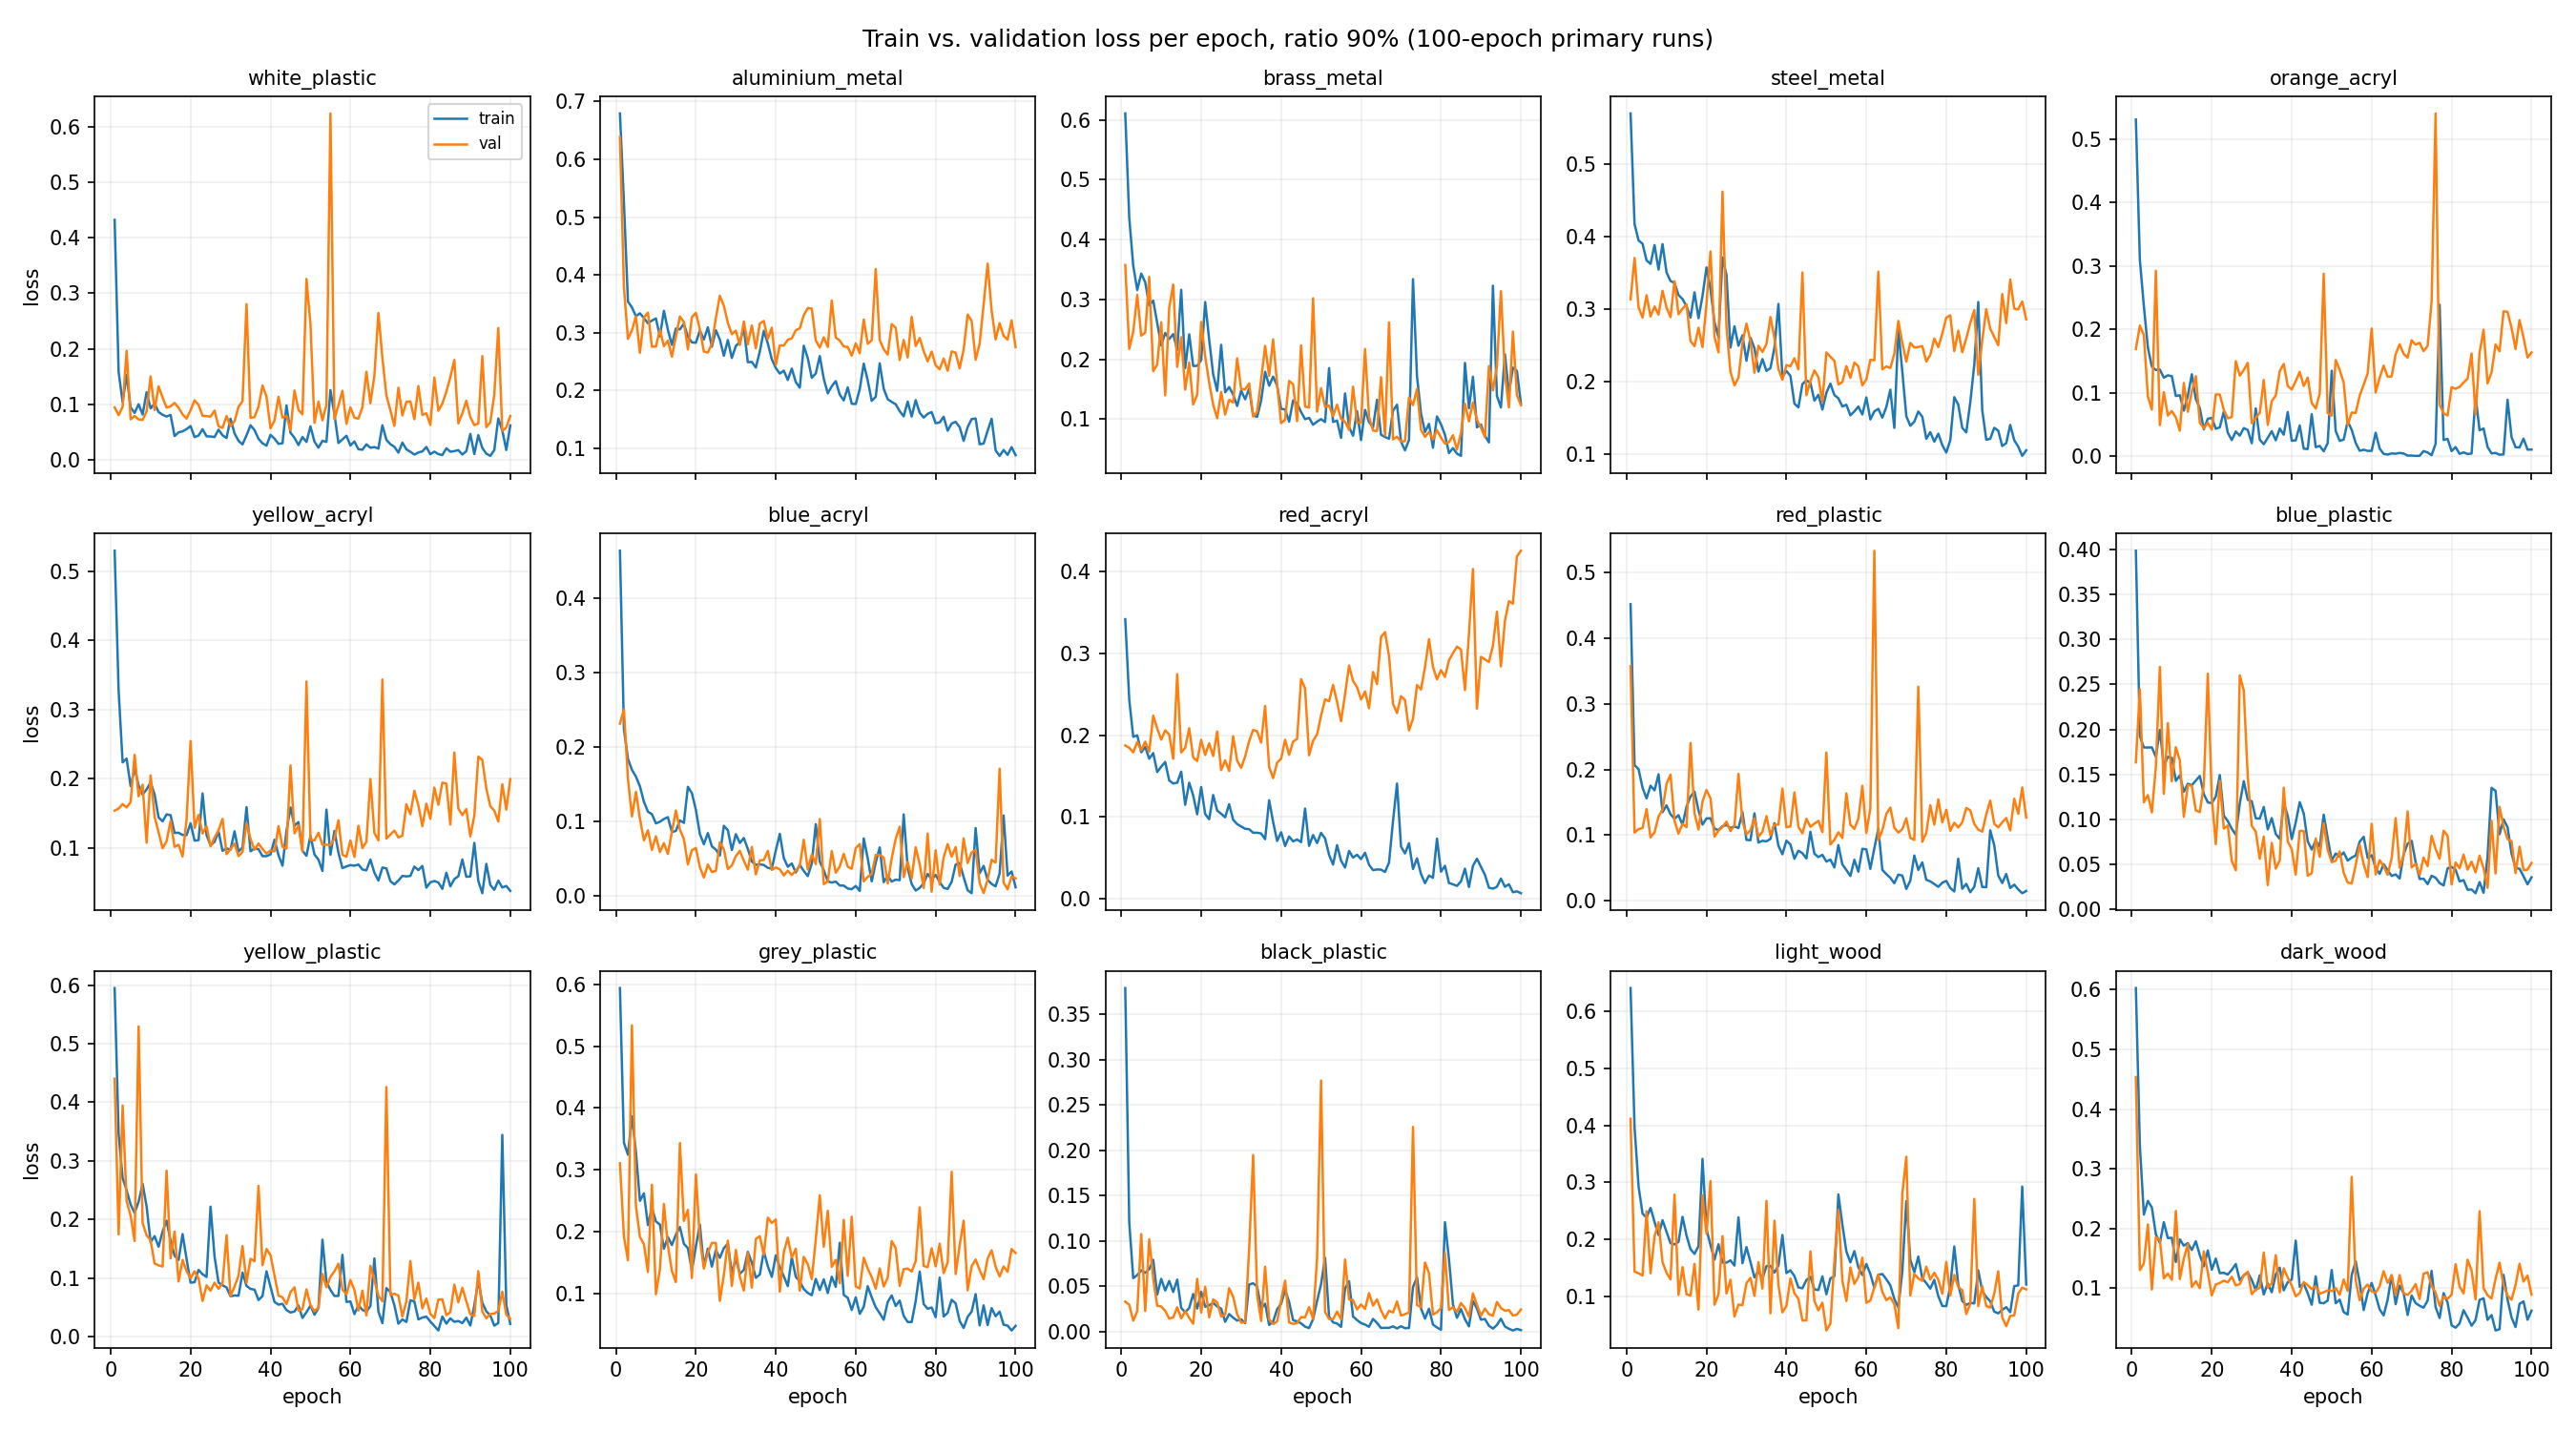
\includegraphics[width=\textwidth]{fig_loss_curves_ratio90.png}
\caption{Training (blue) and validation (orange) loss per epoch, for all 15 materials at
the $90\%$ O2I ratio, over the full 100-epoch primary training run. Validation loss is
visibly noisier than training loss throughout, consistent with the smaller size of the
validation split relative to the training split.}
\label{fig:loss-curves}
\end{figure}

Most materials show the expected pattern for a network trained from scratch (i.e.\ without
an ImageNet-pretrained head start, per the supervisor's instruction,
Section~\ref{sec:methodology-training}): a rapid initial drop in both losses over the
first $5$--$10$ epochs, followed by a slower, noisy decline, with validation loss
consistently above and noisier than training loss but not diverging from it. Black
plastic and brass metal show the cleanest, most stable convergence of the 15, with both
curves settling to a low, stable value by roughly epoch 40. Red acryl is the clearest
counter-example: its training loss continues falling smoothly toward zero across all 100
epochs, but its validation loss reaches a minimum around epoch 20--30 and then rises
steadily for the remainder of training, ending roughly twice as high as its minimum --
textbook overfitting, where the network increasingly memorises training-specific detail
that does not generalise to unseen validation crops. This is precisely the failure mode
that the project's F1-based checkpointing strategy (\texttt{BEST\_METRIC = "f1"},
Section~\ref{sec:methodology-training}) is designed to guard against: rather than using
the final epoch's weights, training keeps the checkpoint from whichever epoch achieved the
best validation F1 score, which for red acryl falls well before this later overfitting
sets in. Inspecting these curves therefore serves two purposes at once: it confirms that
no model's reported result was undermined by a training run that diverged or failed to
converge, and it demonstrates concretely, on a real example, why checkpoint selection by
validation F1 rather than by final epoch was the correct design choice for a
from-scratch, non-pretrained CNN.

\subsubsection{Primary Result: Test-Set F1 by Material and O2I Ratio}
\label{sec:results-primary-table}

Every number reported up to this point in the thesis -- including every F1 score used for
checkpoint selection during training -- was computed on the \emph{validation} split, which
is correct and expected during development (Section~\ref{sec:methodology-split}), but
means that no number reported so far is a final, once-touched measure of how well these
models actually generalise. Following the project's locked protocol, the test split was
therefore touched exactly once, at this point, purely to compute final performance: each
of the 75 trained checkpoints was loaded and evaluated, in inference only (no further
training, no further decisions made on the basis of the result), on its corresponding
held-out test crops. Table~\ref{tab:ovr-full-results} reports the resulting test-set F1
score for every (material, ratio) combination -- the primary quantitative result of Phase
2 of this thesis.

\begin{table}[h]
\centering
\footnotesize
\begin{tabular}{lccccc}
\hline
\textbf{Material} & \textbf{90\%} & \textbf{70\%} & \textbf{50\%} & \textbf{30\%} & \textbf{10\%} \\
\hline
White plastic   & 0.94 & 0.87 & 0.86 & 0.81 & 0.88 \\
Aluminium metal & 0.61 & 0.59 & 0.51 & 0.33 & 0.39 \\
Brass metal     & 0.91 & 0.85 & 0.84 & 0.94 & 0.77 \\
Steel metal     & 0.52 & 0.47 & 0.56 & 0.53 & 0.29 \\
Orange acryl    & 0.82 & 0.89 & 0.81 & 0.73 & 0.76 \\
Yellow acryl    & 0.79 & 0.87 & 0.85 & 0.78 & 0.69 \\
Blue acryl      & 0.96 & 0.98 & 0.94 & 0.96 & 0.91 \\
Red acryl       & 0.79 & 0.75 & 0.74 & 0.64 & 0.64 \\
Red plastic     & 0.85 & 0.83 & 0.70 & 0.71 & 0.65 \\
Blue plastic    & 0.94 & 0.96 & 0.90 & 0.92 & 0.82 \\
Yellow plastic  & 0.88 & 0.86 & 0.94 & 0.91 & 0.89 \\
Grey plastic    & 0.77 & 0.82 & 0.70 & 0.74 & 0.64 \\
Black plastic   & 0.90 & 0.96 & 0.96 & 0.96 & 0.94 \\
Light wood      & 0.78 & 0.71 & 0.83 & 0.74 & 0.73 \\
Dark wood       & 0.84 & 0.81 & 0.81 & 0.83 & 0.82 \\
\hline
\textbf{Mean} & \textbf{0.820} & \textbf{0.816} & \textbf{0.796} & \textbf{0.769} & \textbf{0.720} \\
\hline
\end{tabular}
\caption{Test-set F1 score for all 75 one-vs-rest models (15 materials $\times$ 5 O2I
ratios), computed once, after training, on the held-out test split. The bottom row is the
mean across all 15 materials at each ratio.}
\label{tab:ovr-full-results}
\end{table}

The mean F1 score across all 15 materials declines monotonically and, notably,
\emph{accelerates} as the O2I ratio shrinks: from $0.820$ at a $90\%$ ratio, the mean falls
only slightly to $0.816$ at $70\%$ and $0.796$ at $50\%$, before dropping more steeply to
$0.769$ at $30\%$ and $0.720$ at $10\%$. Taken at face value, this is already a direct,
classification-level answer to part of the thesis's research question: shrinking the
object relative to the frame measurably degrades classification accuracy, and the
complex factory background is the only thing left to fill the remaining space, so this
decline is consistent with the background increasingly interfering with classification
as the object shrinks. Figure~\ref{fig:f1-per-material} and Figure~\ref{fig:f1-heatmap}
visualise this same result in two complementary ways.

\begin{figure}[h]
\centering
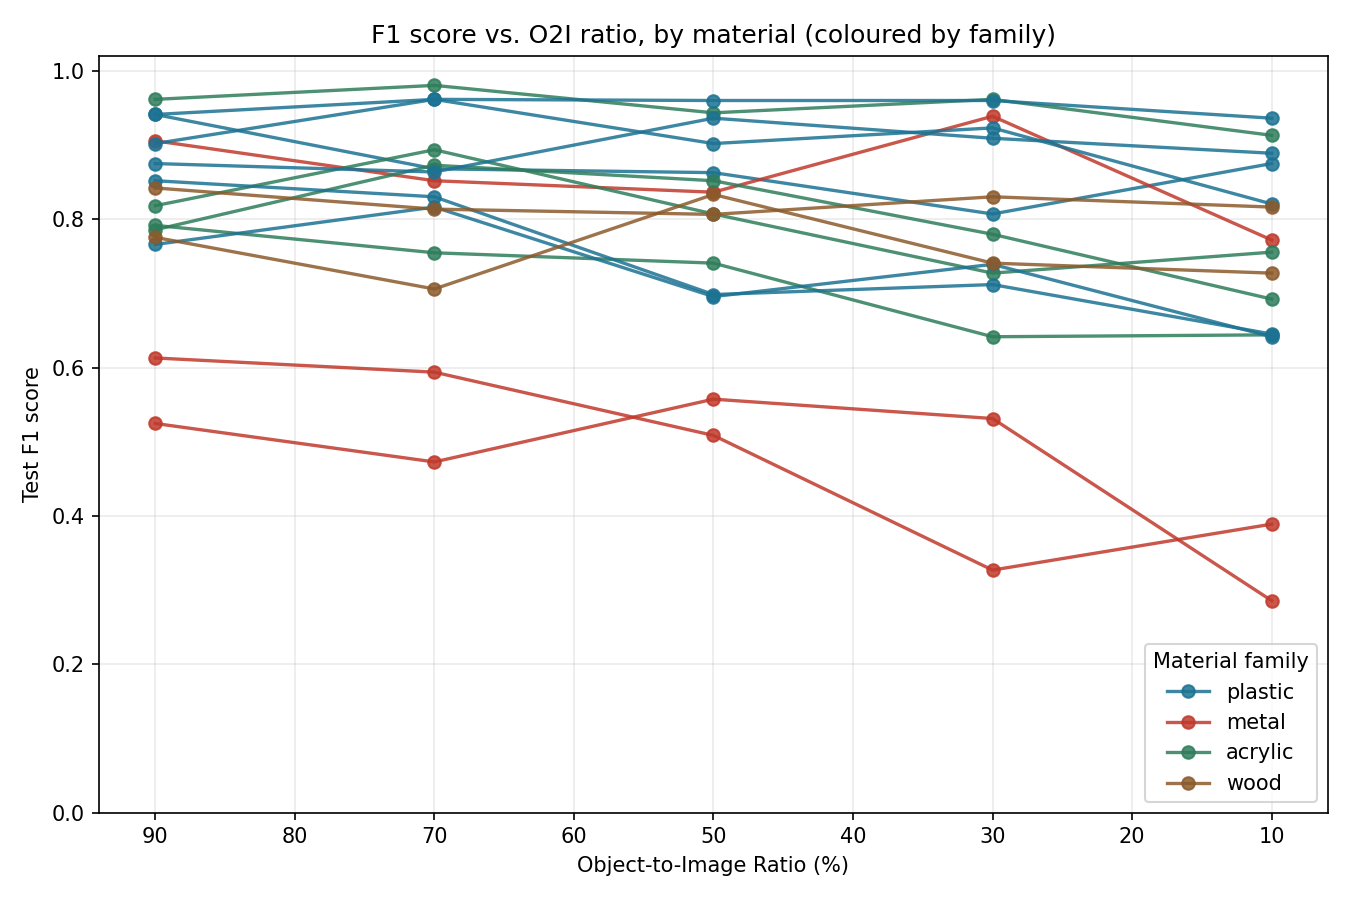
\includegraphics[width=0.85\textwidth]{fig_f1_per_material.png}
\caption{Test F1 score against O2I ratio for all 15 materials, coloured by material
family (plastic, metal, acrylic, wood). Most materials cluster in a band between roughly
$0.7$ and $0.95$ F1 with a gentle downward slope; the two bare, reflective metals
(aluminium, steel; red) are visibly separated below this band at every ratio.}
\label{fig:f1-per-material}
\end{figure}

\begin{figure}[h]
\centering
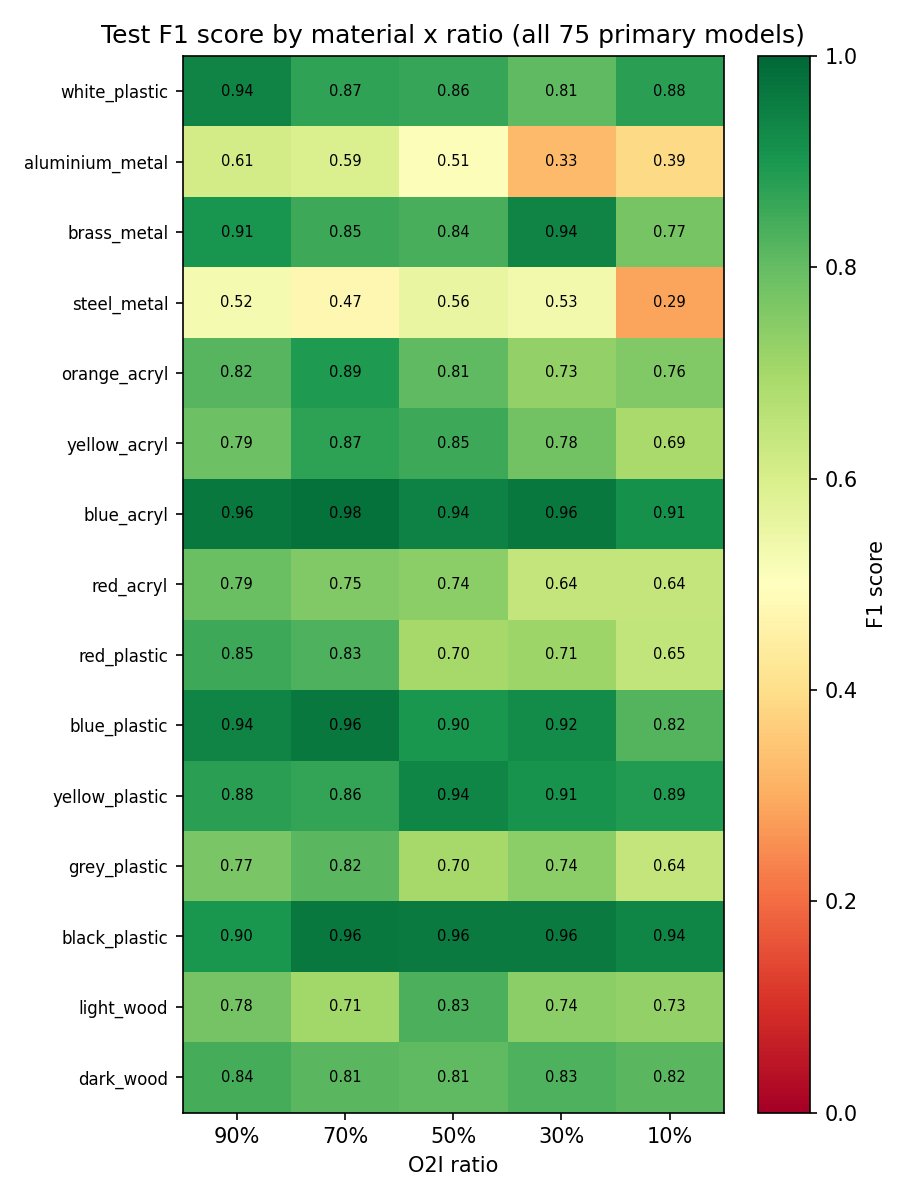
\includegraphics[width=0.6\textwidth]{fig_f1_heatmap.png}
\caption{The same 75 test F1 scores as Table~\ref{tab:ovr-full-results}, shown as a
material $\times$ ratio heatmap (green = high F1, red = low F1). The two metal rows
(aluminium, steel) stand out as a visibly weaker band across all five ratios, rather than
only at low ratios.}
\label{fig:f1-heatmap}
\end{figure}

Figure~\ref{fig:f1-per-material} makes visible a pattern the mean alone does not: the
decline is not uniform across materials. Several materials are almost flat across the
full ratio range -- black plastic stays between $0.90$ and $0.96$ F1 at every ratio, and
blue acryl between $0.91$ and $0.98$ -- while the two bare metals, aluminium and steel,
sit well below every other material at \emph{every} ratio, including $90\%$, where the
object fills most of the frame and background interference should, in principle, be
minimal. This is an important qualification of the headline ratio-decline finding: for
most materials, weak performance at low ratios is plausibly explained by background
dominance in the way the research question anticipates, but for aluminium and steel, poor
performance is already present when the object is large, which a pure O2I-ratio
explanation cannot account for on its own. Section~\ref{sec:results-qualitative}
investigates this anomaly directly using the occlusion sensitivity and Grad-CAM overlays,
and finds that the two metals fail for two genuinely different underlying reasons.

\subsection{Headline Finding: Occlusion Sensitivity and Grad-CAM Disagree}
\label{sec:results-divergence}

The explainability pipeline (Section~\ref{sec:methodology-explainability}) was run across
all 75 models, producing $750$ image analyses per method. Table~\ref{tab:centerfrac}
reports the mean $\text{center\_frac}$ (Section~\ref{sec:methodology-centerfrac}), averaged
across all 15 materials, at each of the five O2I ratios.

\begin{table}[h]
\centering
\begin{tabular}{lcc}
\hline
\textbf{O2I ratio} & \textbf{Occlusion sensitivity} & \textbf{Grad-CAM} \\
\hline
90\% & 0.556 & 0.709 \\
70\% & 0.582 & 0.657 \\
50\% & 0.612 & 0.672 \\
30\% & 0.661 & 0.627 \\
10\% & 0.721 & 0.407 \\
\hline
\end{tabular}
\caption{Mean $\text{center\_frac}$ by O2I ratio and explainability method, averaged
across all 15 materials (750 image analyses per method).}
\label{tab:centerfrac}
\end{table}

Grad-CAM shows the pattern the research question predicts: as the object shrinks from a
$90\%$ to a $10\%$ ratio, its $\text{center\_frac}$ falls from $0.709$ to $0.407$, meaning
the network's internal evidence increasingly originates outside the (shrinking) object
region as the background comes to dominate the frame. Occlusion sensitivity shows the
\emph{opposite} trend over the same range, rising from $0.556$ to $0.721$ -- reading as
\emph{more} object-focused, not less, precisely where Grad-CAM reads the model as
increasingly background-reliant. Both methods were applied to the same trained models on
the same sampled images, so this divergence is not attributable to a difference in what
was measured, only to how each method measures it.

This divergence is explained by a structural difference between the two methods rather
than by either one being faulty. Grad-CAM (Section~\ref{sec:background-gradcam}) computes
a single gradient over the \emph{entire} final feature map at once, so if the network
relies on the background as a whole -- not on any one specific spot, but on the general,
repeated presence of factory structure throughout the frame -- this holistic computation
is positioned to detect it. Occlusion sensitivity (Section~\ref{sec:background-occlusion}),
by contrast, is a strictly local, one-patch-at-a-time test. At a low O2I ratio, the object
occupies only a small region of the frame, so a single occluded patch can cover a large
fraction of the network's only concentrated positive evidence, producing a large,
easily-detected score change exactly at the object's location. The background, however, is
large and visually repetitive (the same conveyor, cables, and sensors recur throughout the
frame), so removing any \emph{one} patch of it leaves visually similar background fully
intact elsewhere in the image, and the measured effect of that single removal is small even
when the network genuinely depends on the background as a whole. Patch-based occlusion
sensitivity is therefore structurally insensitive to distributed reliance on redundant
background information, a limitation Grad-CAM does not share. This is developed further,
with reference to the wider explainability literature, in
Section~\ref{sec:discussion}.

\subsubsection{Qualitative Evidence: Occlusion and Grad-CAM Overlays}
\label{sec:results-qualitative}

Table~\ref{tab:centerfrac} reports the divergence between the two methods only as an
aggregate number, averaged over 750 images per method. To make this divergence concrete,
and to investigate the aluminium/steel anomaly surfaced in
Section~\ref{sec:results-primary-table}, this section examines individual occlusion
sensitivity and Grad-CAM overlays for three materials -- black plastic (the strongest,
most ratio-robust performer), and steel metal and aluminium metal (the two weakest
performers at every ratio) -- each shown at a $90\%$ and a $10\%$ O2I ratio. These are
illustrative single-image examples, not aggregate statistics, and are read accordingly:
they are used here to explain \emph{why} the aggregate numbers look the way they do, not
to replace them.

\begin{figure}[h]
\centering
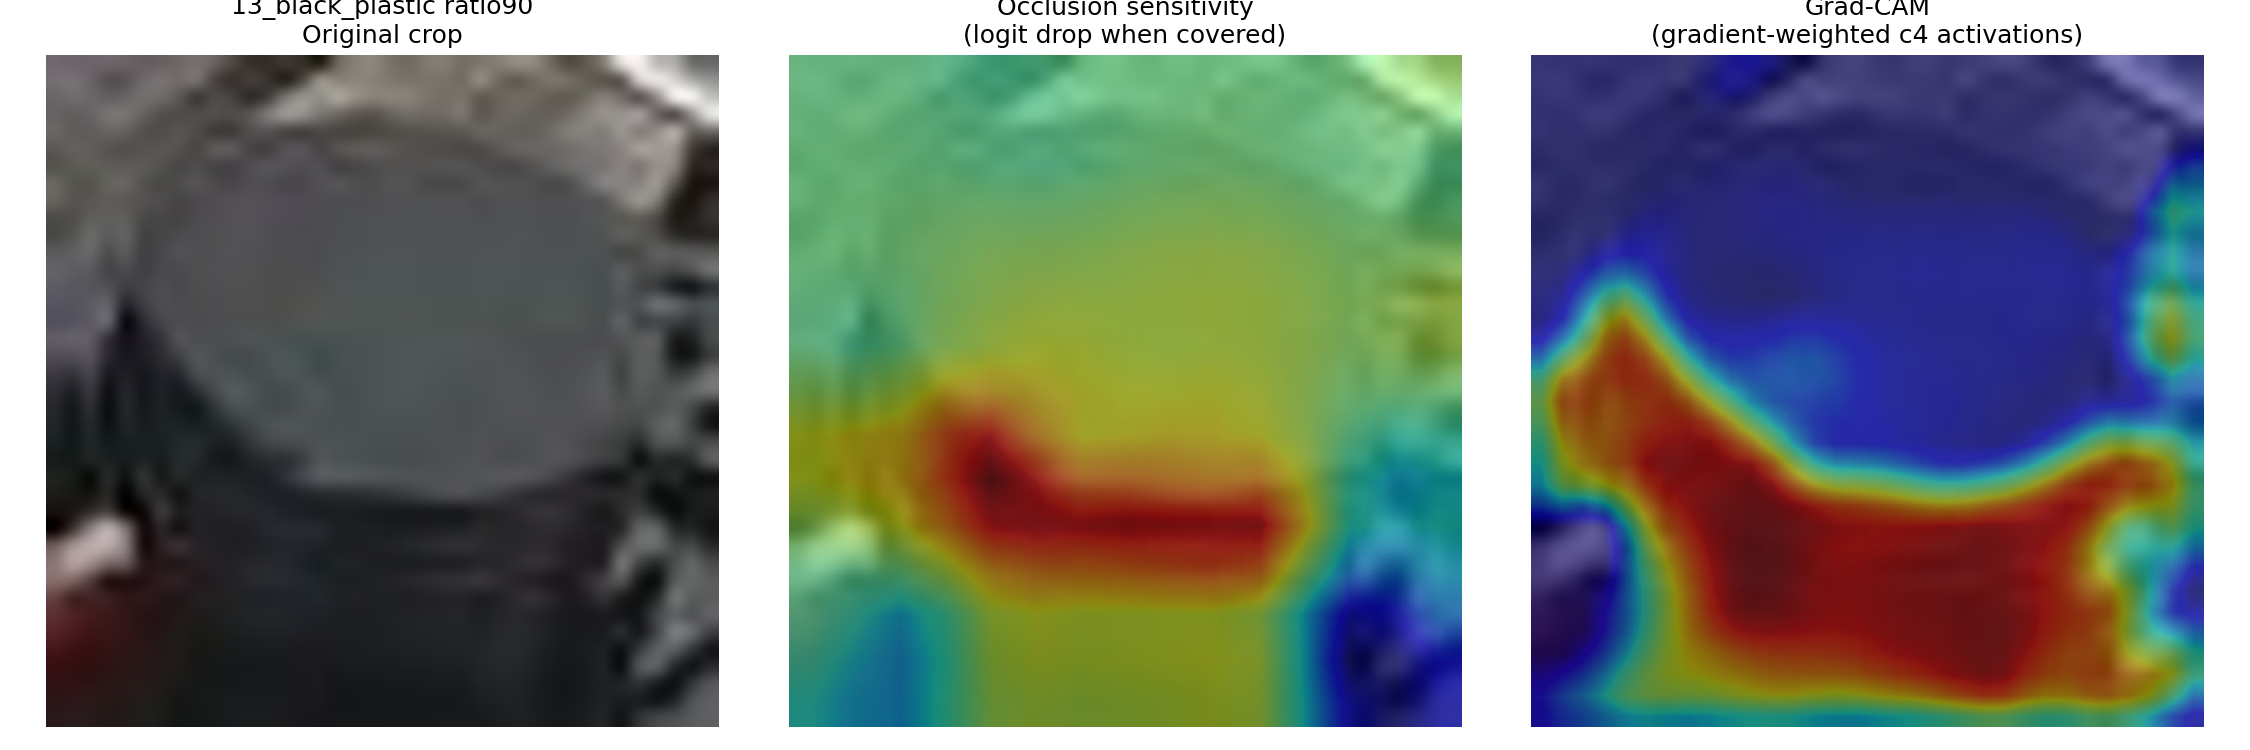
\includegraphics[width=\textwidth]{overlay_blackplastic_r90.png}
\caption{Black plastic, $90\%$ O2I ratio. Left: the original crop. Centre: occlusion
sensitivity (red = large logit drop when that patch is covered, i.e.\ the model relies on
it). Right: Grad-CAM (red = strong gradient-weighted activation). Both methods concentrate
on the same horizontal reflective highlight running across the workpiece's top surface --
a real, discriminative visual feature of this material's surface finish, not a background
artefact.}
\label{fig:overlay-black-r90}
\end{figure}

\begin{figure}[h]
\centering
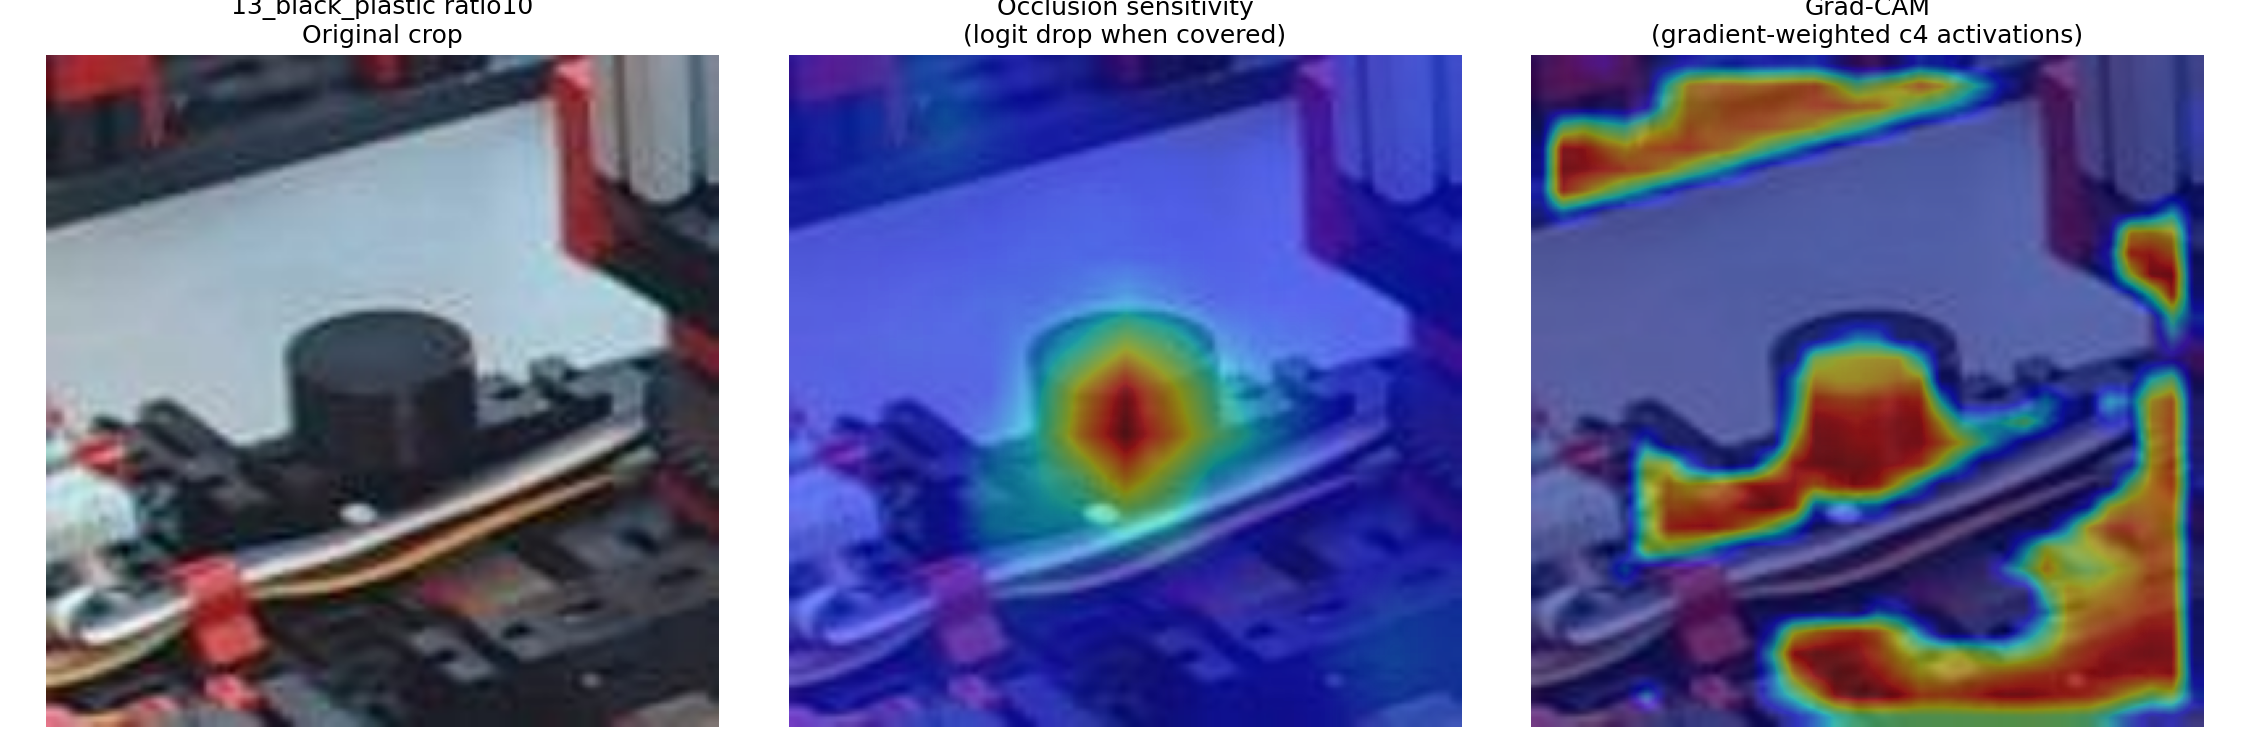
\includegraphics[width=\textwidth]{overlay_blackplastic_r10.png}
\caption{Black plastic, $10\%$ O2I ratio. Despite the object now occupying only a small
fraction of a visually busy frame (conveyor structure, metal brackets, another
workpiece), occlusion sensitivity forms a tight, sharply concentrated hotspot almost
exactly on the object, and Grad-CAM likewise concentrates its strongest activation on the
object and the bracket directly beneath it, with only minor spread into the surrounding
frame corners.}
\label{fig:overlay-black-r10}
\end{figure}

Black plastic's overlays are consistent with its near-flat F1 curve
(Figure~\ref{fig:f1-per-material}): even at a $10\%$ ratio, where background pixels
outnumber object pixels roughly nine to one, both explainability methods agree that the
network's decision is still substantially driven by the object itself. This is the
``well-behaved'' case the research question implicitly assumes as a baseline -- a material
whose visual signature is distinctive enough that the network continues to find and use
it even as the object shrinks.

\begin{figure}[h]
\centering
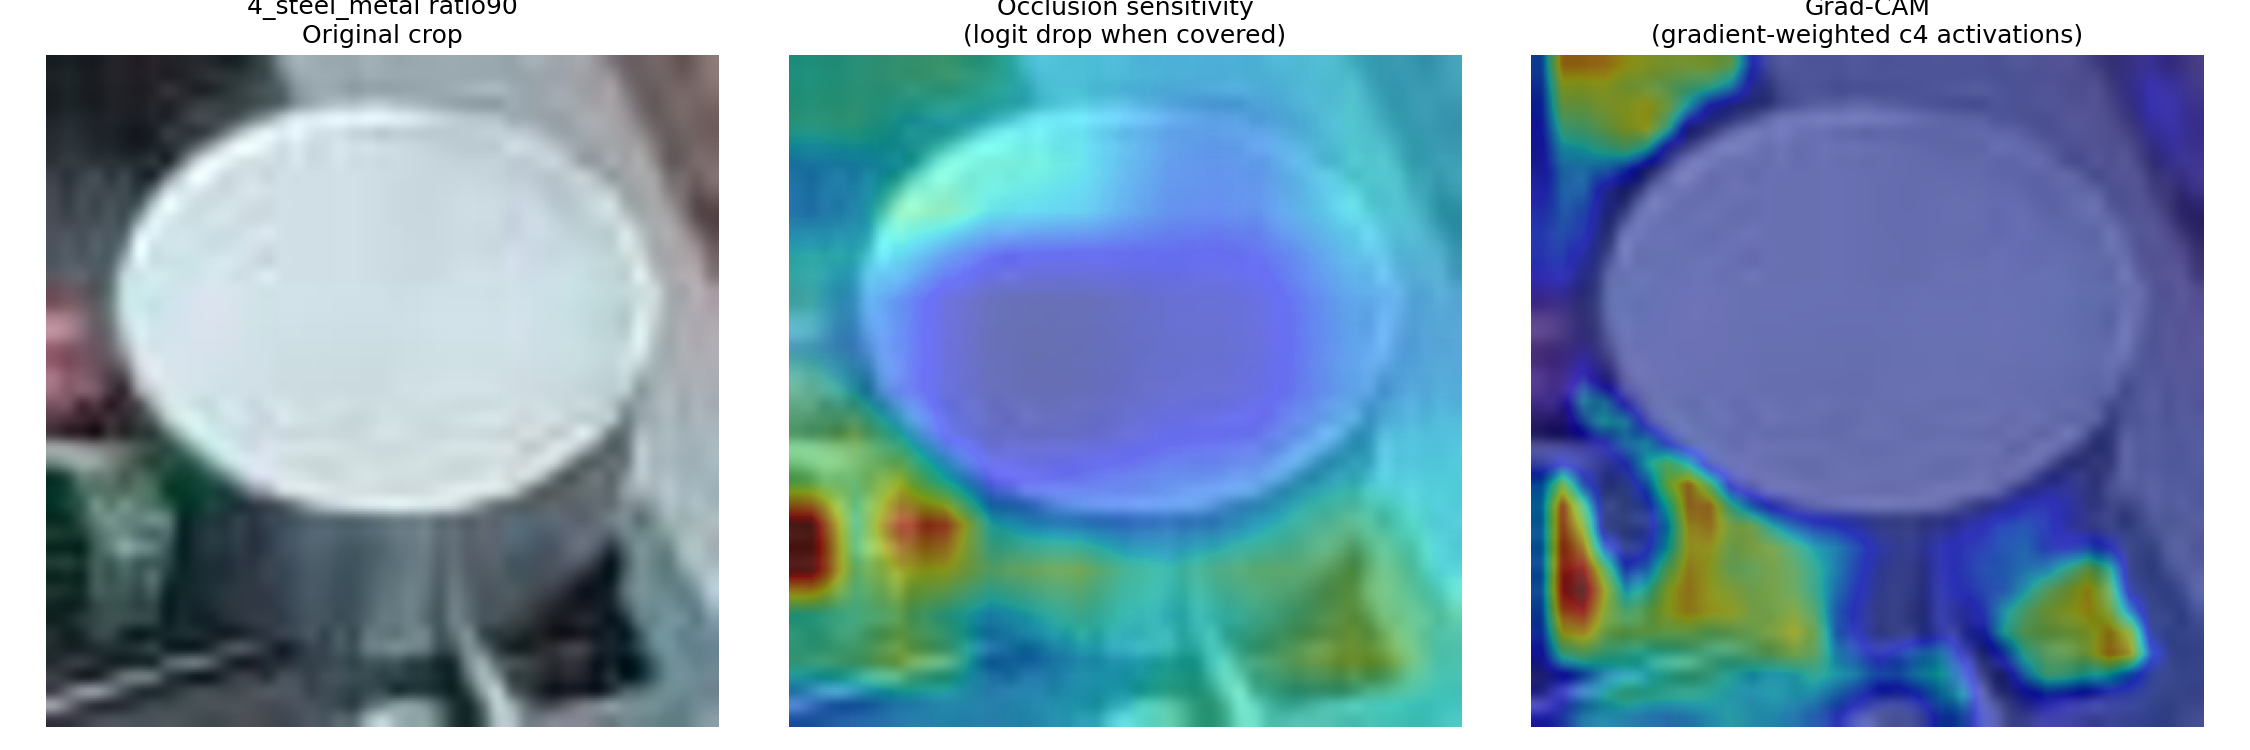
\includegraphics[width=\textwidth]{overlay_steelmetal_r90.png}
\caption{Steel metal, $90\%$ O2I ratio. The object fills most of the frame, yet both
occlusion sensitivity and Grad-CAM show only weak, near-neutral response \emph{on} the
object itself, with the strongest evidence in both maps located off the object, in the
background structure to its lower left.}
\label{fig:overlay-steel-r90}
\end{figure}

\begin{figure}[h]
\centering
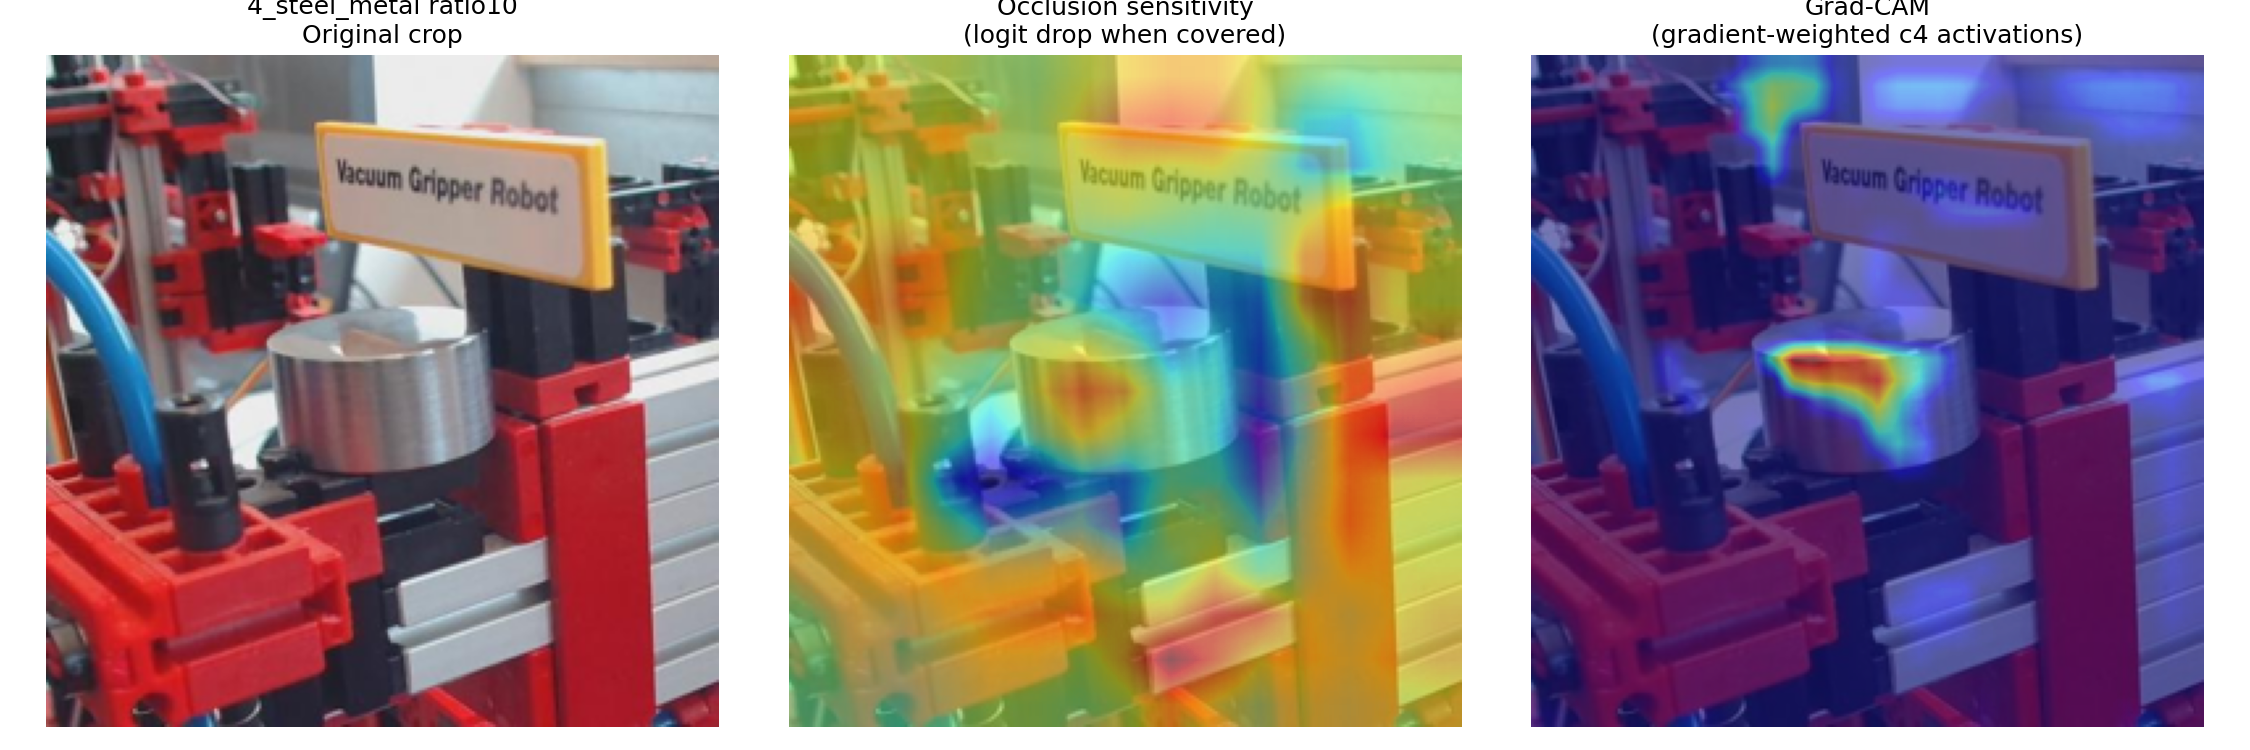
\includegraphics[width=\textwidth]{overlay_steelmetal_r10.png}
\caption{Steel metal, $10\%$ O2I ratio, in a scene containing the factory's ``Vacuum
Gripper Robot'' signage. Occlusion sensitivity is diffuse, spreading moderate sensitivity
broadly across much of the frame rather than concentrating sharply; Grad-CAM concentrates
more tightly on the object and the mechanism immediately beneath it.}
\label{fig:overlay-steel-r10}
\end{figure}

Steel metal's overlays explain why this material is the weakest performer in
Table~\ref{tab:ovr-full-results} at \emph{every} ratio, not only low ones.
Figure~\ref{fig:overlay-steel-r90} is the clearest single-image demonstration in this
thesis of background dominance occurring independently of the O2I ratio: with the object
occupying most of the frame, a pure ratio-driven account would predict strong,
object-centred evidence, but both methods instead point at the background. This suggests
that for steel, the factory background is not merely filling otherwise-empty space at low
ratios -- it is actively out-competing the object as a source of evidence even when the
object is large. A plausible physical explanation, consistent with steel's mirror-like,
highly reflective surface, is that the object's own surface appearance is partly a
reflection \emph{of} the surrounding factory environment, so the boundary between
``object'' and ``background'' information is less clean for this material than for a
matte plastic. Note, however, that Figure~\ref{fig:overlay-steel-r10} does not show a
simple continuation of this trend to an even more background-dominated state at the
lowest ratio -- if anything, Grad-CAM concentrates more on the object at $10\%$ than at
$90\%$ in this particular pair of sampled images. Given that each figure here is a single
illustrative example rather than an aggregate statistic, this should be read as a sign
that steel's failure mode is more complex than a monotonic ratio effect, not as evidence
against the aggregate trend in Table~\ref{tab:centerfrac}, which remains the statistically
supported result.

\begin{figure}[h]
\centering
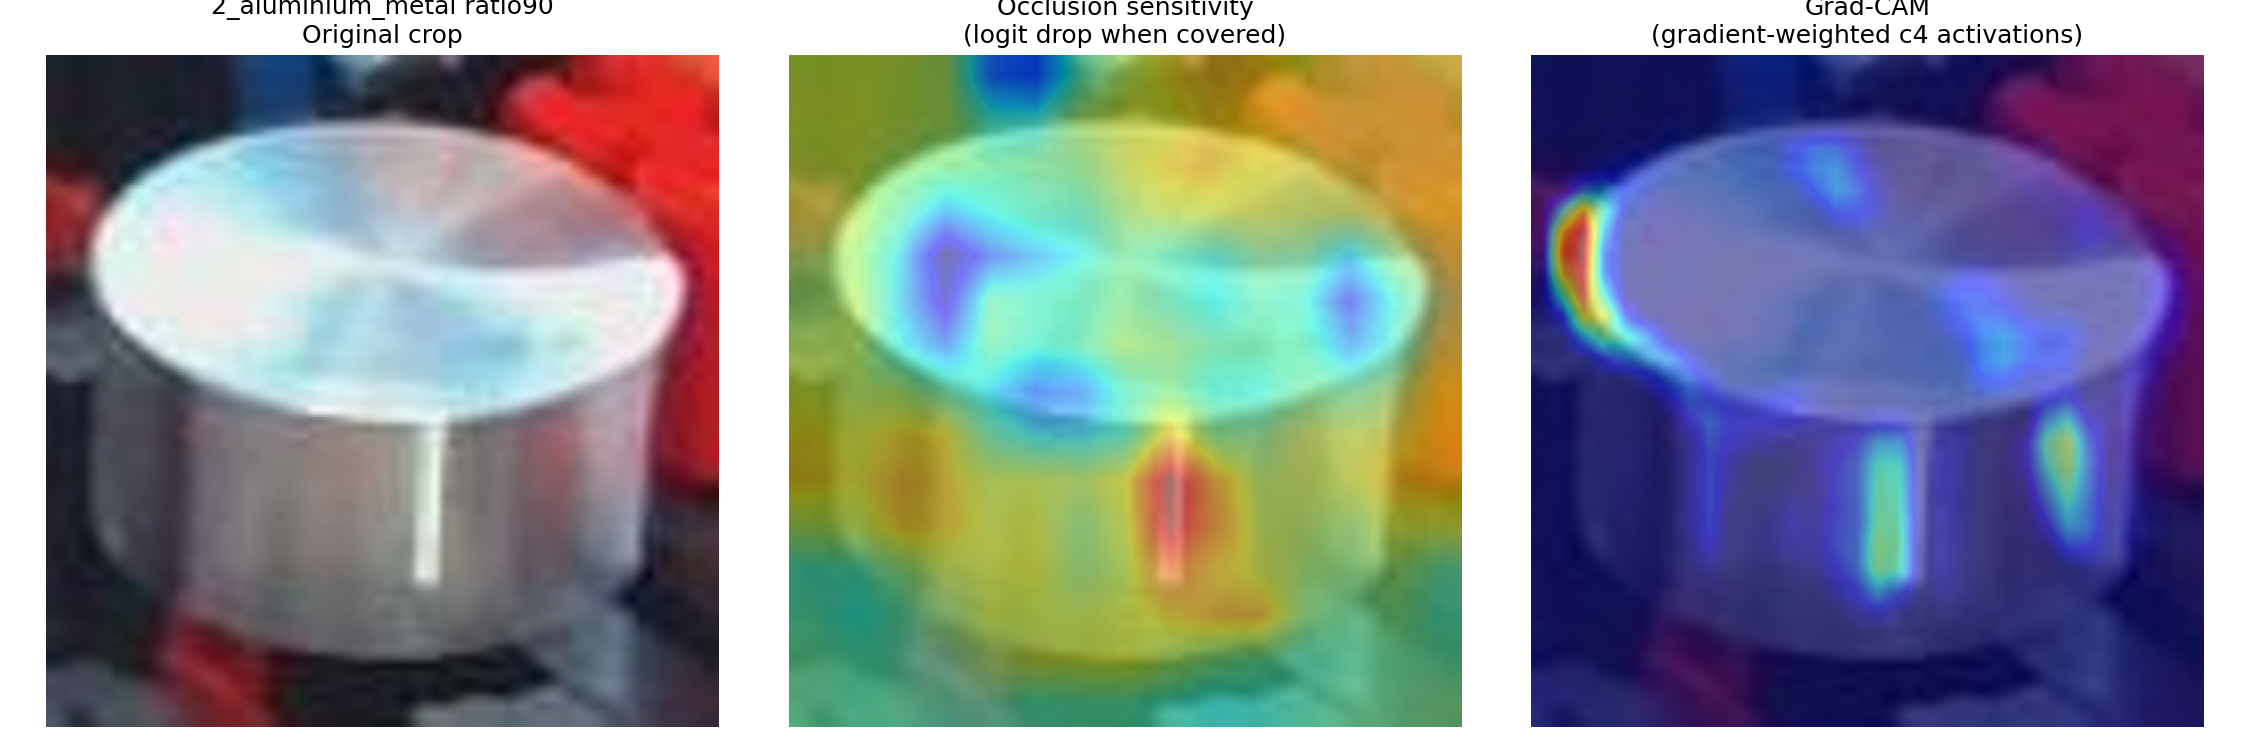
\includegraphics[width=\textwidth]{overlay_aluminiummetal_r90.png}
\caption{Aluminium metal, $90\%$ O2I ratio. Both methods concentrate mainly on or
immediately adjacent to the object -- its rim and a vertical reflective seam on its front
face -- with only modest spread into the neighbouring background structure, unlike the
steel case in Figure~\ref{fig:overlay-steel-r90}.}
\label{fig:overlay-alu-r90}
\end{figure}

\begin{figure}[h]
\centering
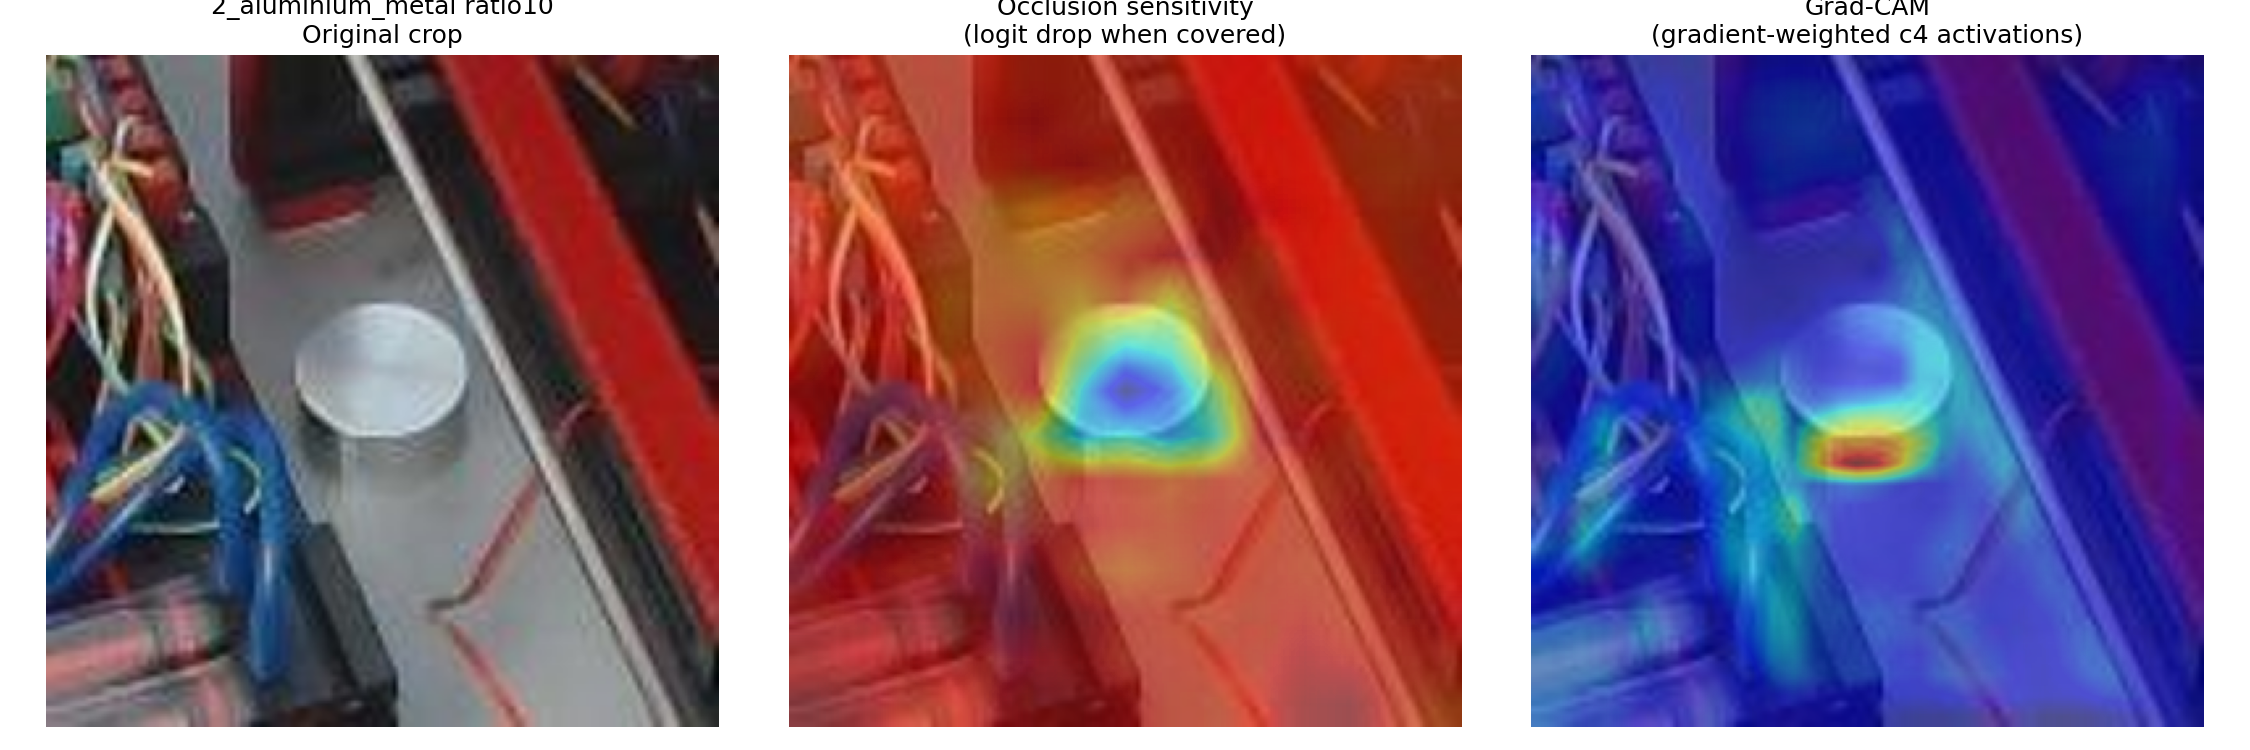
\includegraphics[width=\textwidth]{overlay_aluminiummetal_r10.png}
\caption{Aluminium metal, $10\%$ O2I ratio, amid factory wiring and conveyor rail. Both
methods form a hotspot essentially on the object itself, with only a small secondary
Grad-CAM response on the adjacent wire bundle.}
\label{fig:overlay-alu-r10}
\end{figure}

Aluminium metal is, by Table~\ref{tab:ovr-full-results}, almost as weak a performer as
steel (F1 between $0.33$ and $0.61$ across ratios), yet its overlays tell a visibly
different story: at both ratios shown, both explainability methods remain concentrated on
or very close to the object itself, not on the background. This is a genuinely useful
negative result: it shows that low F1 and background-focused attention are not the same
thing, and that the explainability pipeline can tell them apart. If aluminium's weak
classification were caused by background dominance in the way steel's appears to be, its
overlays should look like steel's; they do not. A more plausible explanation for
aluminium's weakness is instability in the object's \emph{own} visual signature rather
than reliance on the background: aluminium's polished surface reflects whatever
surrounds it (different conveyor sections, different lighting, nearby coloured parts),
so two aluminium crops can look quite different from each other even though the network
is correctly attending to the object in both. This would manifest as poor
material-versus-material discriminability despite good object localisation -- exactly
the pattern observed here. Steel and aluminium therefore illustrate two distinct failure
modes that happen to produce similarly poor F1 scores: steel's evidence-generation
apparatus reaches outside the object into the background, while aluminium's stays on the
object but the object's own appearance is an unreliable signal. Section~\ref{sec:discussion-material}
returns to this distinction.

\subsection{Robustness Checks}
\label{sec:results-robustness}

Before accepting the finding in Section~\ref{sec:results-divergence} as reliable, two
potential threats to its validity were investigated directly rather than assumed away.

\subsubsection{Grad-CAM Degeneracy}
\label{sec:results-degeneracy}

Grad-CAM is known to occasionally produce a completely flat, uninformative heatmap when
its ReLU step zeroes out every channel's contribution for a given image
(Section~\ref{sec:background-gradcam}). This occurred in $172$ of the $750$ analyses
($23\%$), with a strongly material-dependent rate: as low as $0\%$ for black plastic and
$2\%$ for brass metal and steel metal, but as high as $74\%$ for yellow plastic and over
$40\%$ for light wood, orange acryl, blue plastic, and grey plastic. Since a degenerate
heatmap falls back to the neutral $\text{center\_frac} = 0.5$
(Section~\ref{sec:methodology-centerfrac}), a concern is whether this degeneracy rate
could itself be manufacturing the downward Grad-CAM trend in Table~\ref{tab:centerfrac} --
for example, if degeneracy became more common at low ratios, pulling the mean toward the
neutral $0.5$ value in a way that mimicked a genuine shift toward the background. Checking
the degeneracy rate by ratio directly rules this out: $17\%$ (ratio 90), $27\%$ (ratio 70),
$17\%$ (ratio 50), $23\%$ (ratio 30), and $29\%$ (ratio 10) -- a mild increase at the
lowest ratio, but far too small and unevenly distributed across the middle ratios to
account for a shift from $0.709$ to $0.407$. The aggregate Grad-CAM trend in
Table~\ref{tab:centerfrac} is therefore not an artefact of degenerate heatmaps, though
per-material Grad-CAM results for the highest-degeneracy materials listed above should be
interpreted with this caveat in mind.

\subsubsection{Crop-Centering Validation}
\label{sec:results-centering}

The $\text{center\_frac}$ metric (Section~\ref{sec:methodology-centerfrac}) assumes the
object is centred within its crop; if this assumption failed, especially at low ratios
where the central box is small, the metric would be unreliable regardless of which
explainability method it is applied to. This was checked two ways: first, by reading the
crop-generation code directly, which crops symmetrically around the bounding-box centre
and therefore guarantees centering by construction rather than by approximation; second,
by directly measuring the object's pixel centroid on real sample crops, which confirmed an
offset of under $2\%$ of the crop dimension from true centre. The centering assumption
underlying $\text{center\_frac}$ is therefore confirmed to hold.

\subsection{Supplementary Investigation: Extended Training at 200 Epochs}
\label{sec:results-200epoch}

The primary results in this thesis use 100 training epochs
(Section~\ref{sec:methodology-training}). To check whether 100 epochs under-trained any
model, this investigation proceeded in two stages. First, three materials -- aluminium,
grey plastic, and steel metal -- were retrained for 200 epochs at all five O2I ratios (15
additional runs), chosen as an initial, quicker check spanning the primary results'
weakest performer (steel), a mid-table performer (grey plastic), and what turned out to be
the most severely undertrained material (aluminium). Table~\ref{tab:200epoch} reports this
first-stage result in detail, read row by row below, since walking through it concretely
motivated the second stage: extending the same check to the remaining 12 materials, which
Section~\ref{sec:results-200epoch-full} reports.

\begin{table}[h]
\centering
\footnotesize
\setlength{\tabcolsep}{4pt}
\begin{tabular}{p{2.1cm}cccccp{4cm}}
\hline
\textbf{Material} & \textbf{Ratio} & \textbf{F1@100} & \textbf{F1@200} & \textbf{Best ep.@200} & \textbf{$\Delta$} & \textbf{Interpretation} \\
\hline
Aluminium & 90\% & 0.588 & 0.698 & 168 & +0.110 & Large, genuine gain \\
Aluminium & 70\% & 0.597 & 0.756 & 198 & +0.159 & Large, genuine gain \\
Aluminium & 50\% & 0.615 & 0.741 & 159 & +0.126 & Large, genuine gain \\
Aluminium & 30\% & 0.432 & 0.607 & 197 & +0.175 & Largest gain; clearly undertrained at 100 \\
Aluminium & 10\% & 0.480 & 0.625 & 174 & +0.145 & Large, genuine gain \\
Grey plastic & 90\% & 0.824 & 0.857 & 147 & +0.033 & Moderate gain \\
Grey plastic & 70\% & 0.808 & 0.880 & 180 & +0.072 & Moderate gain \\
Grey plastic & 50\% & 0.808 & 0.830 & 194 & +0.022 & Small gain \\
Grey plastic & 30\% & 0.792 & 0.851 & 118 & +0.059 & Moderate gain \\
Grey plastic & 10\% & 0.723 & 0.829 & 199 & +0.106 & Large gain \\
Steel metal & 90\% & 0.702 & 0.700 & 161 & $\approx$0.000 & Flat; already converged \\
Steel metal & 70\% & 0.750 & 0.667 & 85 & $-$0.083 & Noisy outlier (see below) \\
Steel metal & 50\% & 0.702 & 0.735 & 130 & +0.033 & Moderate gain \\
Steel metal & 30\% & 0.632 & 0.652 & 182 & +0.021 & Small gain \\
Steel metal & 10\% & 0.480 & 0.564 & 173 & +0.084 & Moderate gain \\
\hline
\end{tabular}
\caption{200-epoch supplementary investigation. F1@100 is the original, once-recorded
baseline; F1@200 is the best F1 achieved across the full 200-epoch run; $\Delta$ is the
difference.}
\label{tab:200epoch}
\end{table}

Aluminium shows a large, consistent improvement at every ratio (+0.110 to +0.175),
indicating it was clearly undertrained at 100 epochs. Grey plastic shows a smaller but
still real and consistent improvement across all five ratios (+0.022 to +0.106). Steel
metal is not uniformly flat, contrary to an earlier, more limited observation based on
only two of its five ratios: ratio 90 shows no meaningful change, but ratios 50, 30, and 10
all show real, moderate gains, while ratio 70 shows an apparent \emph{drop}. This drop was
investigated rather than reported at face value: the ratio-70 rerun's own best F1 across
the \emph{entire} 200-epoch run occurred at epoch 85, before it had even reached epoch
100, and nothing in epochs 100--200 improved on it. This means the apparent drop is not a
case of additional training making the model worse (there is no overfitting-past-100
pattern in this run); rather, this particular training run underperformed the original run
from early on, most plausibly due to ordinary run-to-run numerical noise in GPU-based
training (e.g.\ from non-deterministic convolution algorithm selection) rather than any
systematic effect of extended training. It is reported here with this caveat explicit,
rather than as an unqualified $-0.083$ that would misleadingly suggest more training hurts
performance.

\subsubsection{Extending the Check to All 15 Materials}
\label{sec:results-200epoch-full}

The remaining 12 materials were subsequently retrained for 200 epochs at all five O2I
ratios as well (60 further runs), completing the check for the full primary result set.
Table~\ref{tab:200epoch-full} reports the resulting improvement, $\Delta = F1@200 -
F1@100$, for all 75 (material, ratio) combinations. A dagger ($\dagger$) marks a cell
where the 200-epoch run's own best F1 was reached before epoch 100 -- meaning that
particular run's peak occurred within what would have been the original 100-epoch window,
so its $\Delta$ cannot be attributed to the extra epochs at all and instead reflects
ordinary run-to-run training noise (the same situation already identified and explained
for steel metal at a $70\%$ ratio, immediately above). $19$ of the $75$ cells ($25\%$) are
flagged this way and are not over-interpreted individually.

\begin{table}[h]
\centering
\footnotesize
\setlength{\tabcolsep}{4pt}
\begin{tabular}{lccccc}
\hline
\textbf{Material} & \textbf{90\%} & \textbf{70\%} & \textbf{50\%} & \textbf{30\%} & \textbf{10\%} \\
\hline
White Plastic    & +0.017 & +0.000$^\dagger$ & +0.000$^\dagger$ & +0.041 & +0.000$^\dagger$ \\
Aluminium Metal  & +0.110 & +0.159 & +0.125 & +0.175 & +0.145 \\
Brass Metal      & +0.082$^\dagger$ & +0.040 & +0.000$^\dagger$ & +0.023 & +0.062 \\
Steel Metal      & -0.002 & -0.083$^\dagger$ & +0.033 & +0.021 & +0.084 \\
Orange Acryl     & +0.007$^\dagger$ & +0.010$^\dagger$ & +0.000$^\dagger$ & +0.016 & +0.020 \\
Yellow Acryl     & +0.105 & +0.000 & +0.019 & +0.026 & +0.099 \\
Blue Acryl       & +0.000$^\dagger$ & +0.000 & +0.000$^\dagger$ & +0.000$^\dagger$ & +0.021 \\
Red Acryl        & +0.016 & -0.013 & +0.008 & +0.027 & +0.033 \\
Red Plastic      & -0.016 & +0.038 & +0.092 & +0.007 & +0.000$^\dagger$ \\
Blue Plastic     & +0.019 & +0.018 & +0.000$^\dagger$ & +0.057 & +0.000$^\dagger$ \\
Yellow Plastic   & +0.036 & +0.038 & +0.041 & +0.020 & +0.023 \\
Grey Plastic     & +0.034 & +0.072 & +0.022 & +0.059 & +0.106 \\
Black Plastic    & +0.000$^\dagger$ & -0.020$^\dagger$ & +0.000$^\dagger$ & +0.000$^\dagger$ & +0.021 \\
Light Wood       & +0.027 & +0.058 & +0.032 & +0.073 & +0.042 \\
Dark Wood        & +0.032 & +0.005 & +0.048 & +0.018 & +0.048 \\
\hline
\textbf{Mean} & \textbf{+0.031} & \textbf{+0.022} & \textbf{+0.028} & \textbf{+0.037} & \textbf{+0.047} \\
\hline
\end{tabular}
\caption{$\Delta = F1@200 - F1@100$ for all 75 (material, ratio) combinations.
$^\dagger$~marks a cell where the 200-epoch run's own best epoch was below 100, so its
$\Delta$ reflects run-to-run noise rather than a genuine effect of extended training. The
bottom row is the mean $\Delta$ across all 15 materials at each ratio (including
noise-flagged cells, since their errors are as likely to understate as overstate the true
effect and should not be dropped from an average).}
\label{tab:200epoch-full}
\end{table}

Two things stand out. First, the per-material mean $\Delta$ (averaged across all five
ratios) ranks aluminium metal far above every other material at $+0.143$ -- more than
double the next-highest, grey plastic at $+0.059$ -- confirming that the pattern already
visible in the three-material check was not a coincidence of which materials happened to
be chosen first: aluminium is genuinely, substantially undertrained at 100 epochs, more so
than any other material in the study. Most materials cluster in a modest $+0.00$ to
$+0.05$ band (white plastic $+0.012$, blue acryl $+0.004$, orange acryl $+0.010$, black
plastic $+0.000$), indicating they were already close to converged at 100 epochs, which is
consistent with the healthy convergence behaviour observed directly in the loss curves for
most materials in Section~\ref{sec:results-convergence}.

Second, and directly relevant to the aluminium/steel discussion in
Section~\ref{sec:results-qualitative}: steel metal's own mean $\Delta$ is small, $+0.011$
-- close to the well-converged end of the range, not the undertrained end. This is an
important cross-check on that earlier qualitative finding. If steel's weak primary-result
F1 (Table~\ref{tab:ovr-full-results}) were simply an artefact of undertraining, extended
training should have closed much of the gap, the way it did for aluminium; instead, steel
gains almost nothing on average from doubling its training budget. This is independent,
quantitative support for the explanation offered in Section~\ref{sec:results-qualitative}
-- that steel's weakness reflects a genuine background-dominance effect visible in its
occlusion sensitivity and Grad-CAM overlays, not a model that simply needed more time to
train. Aluminium's own case is more nuanced: given its large mean $\Delta$, some of the
weak $100$-epoch F1 that motivated the qualitative analysis in
Section~\ref{sec:results-qualitative} does partly reflect undertraining rather than being
purely explained by an unstable, reflective object signal. However, this does not overturn
that analysis: checking directly, aluminium and steel remain the two lowest-F1 materials
in the entire study at \emph{every} O2I ratio even after 200 epochs of training
(F1@200 ranges $0.607$--$0.756$ for aluminium and $0.564$--$0.735$ for steel, both well
below the $0.76$--$1.00$ range nearly every other material occupies at 200 epochs). Extended
training narrows but does not close the gap between these two bare metals and the rest of
the dataset, so the qualitative distinction drawn between steel and aluminium's failure
modes in Section~\ref{sec:results-qualitative} is read as still standing, with the caveat
that aluminium's 100-epoch numbers specifically should be read as somewhat pessimistic
relative to what a fully-converged aluminium model would achieve.
